%
% Adobe Systems Engineering GmbH - 2014
% Erhan Bagdemir <bagdemir@adobe.com>
%
\documentclass{beamer}

% package declerations
\usepackage[T1]{fontenc}
\usepackage{lmodern}
\usepackage{listings}

\lstset{
        language=Java,
        tabsize=4,
        breaklines=true,
        breakatwhitespace=true,
        escapechar=|,
        basicstyle=\footnotesize\ttfamily,
        numberstyle=\footnotesize\ttfamily,
        aboveskip=\baselineskip,
        captionpos=b,
        columns=fullflexible,
        showstringspaces=false,
        extendedchars=true,
        breaklines=true,
        showtabs=false,
        showspaces=false,
        showstringspaces=false,
        identifierstyle=\ttfamily,
        keywordstyle=\color[rgb]{0.498,0.0,0.333},
        stringstyle=\color[rgb]{0.165,0.0,0.999},
        commentstyle=\color[rgb]{0.247,0.498,0.372}
}

\newcommand\red[1]{\setlength\fboxsep{0pt}\colorbox{red}{\strut #1}}

% theme
\usetheme{torino}

\graphicspath{{./images/}}

% header informations
\author[Bagdemir]{Erhan Bagdemir}
\title{{\fontsize{2em}{1em}\selectfont Lambda Expressions in Java}}
\institute{bagdemir.com - Follow on @ebagdemir}
\setbeamerfont{footnote}{size=\tiny}

% logo of the team.
\titlegraphic{
   
\includegraphics[width=4cm]{duke8}
}

\begin{document}
	\setbeamertemplate{itemize items}[default]
	
	% Cover page.
	\begin{frame}
		\titlepage
		\section{Cover}
	\end{frame}

	% Agenda
	\begin{frame}{Today's Agenda}
		\section{Agenda}
		\begin{columns}
    			\begin{column}{0.3\textwidth}
					\centering
					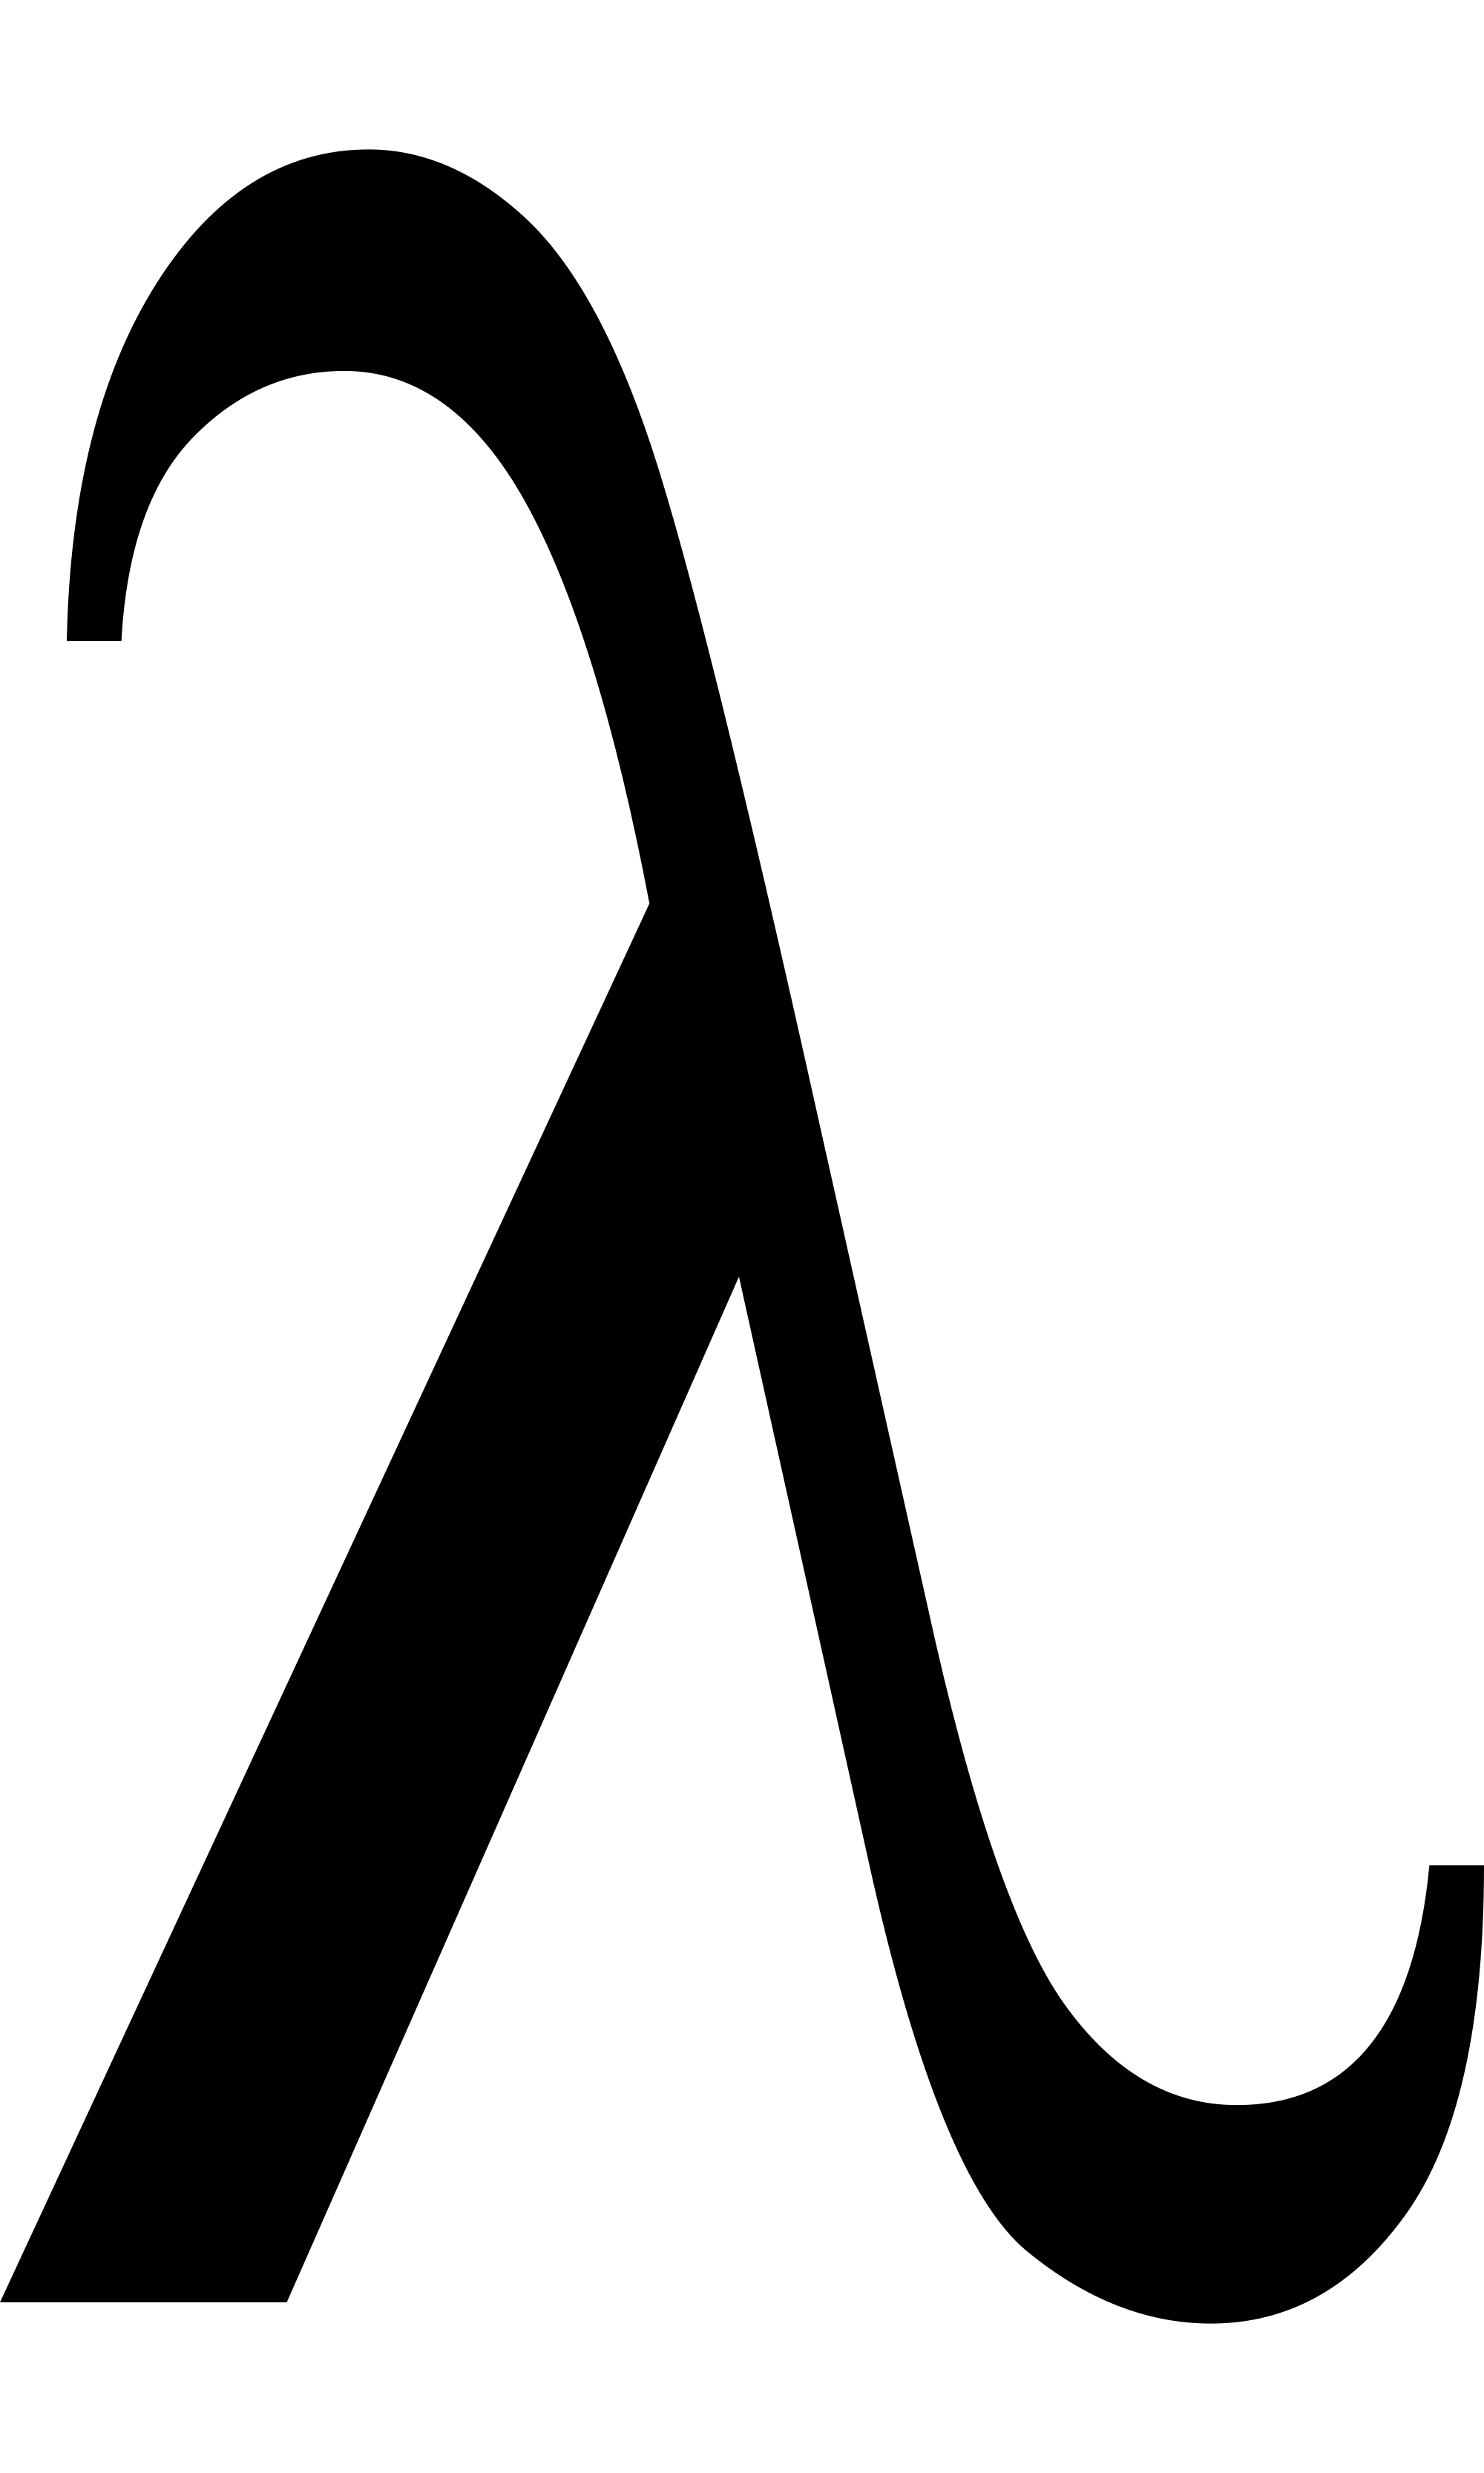
\includegraphics[width=2cm]{lambda}	
    			\end{column}
    			\begin{column}{0.7\textwidth}
    				%	\setbeamertemplate{itemize items}[square]
        				\begin{itemize}
        					\item Definition of Lambda.
        					\item Lambdas in Java.
        					\item Lambdas in ByteCode.
        					\item Lambda examples.
					
							\begin{itemize}
								\item forEach(...) and default implementations
								\item Streams
    	    					\item Parallel Streams.
        					\end{itemize}
					
        				\end{itemize}
    		
    			\end{column}
		\end{columns}
	\end{frame}
	
	\begin{frame}{Lambda Expressions: Definition of Lambda}
		\section{Definition of Lambda}
		\begin{columns}
    			\begin{column}{0.3\textwidth}
					\centering
					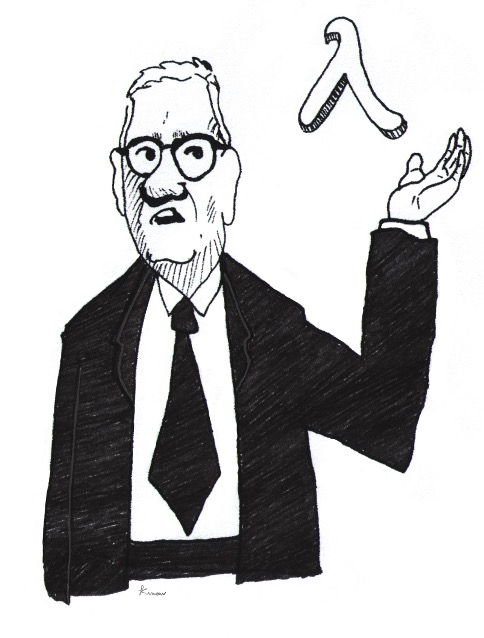
\includegraphics[width=4cm]{church}	
    			\end{column}
    			\begin{column}{0.7\textwidth}
					
					\begin{itemize}
						\item A formal system for expression the computational behaviour.
						\item Invented by Alonzo Church in 1930.	
						\item Lambda expressions consist of many parentheses i.e in Y-combinator:					
					
						\[ Y = \lambda f. (\lambda x. f (x x))(\lambda x. f (x x)) \]
					\end{itemize}
    			\end{column}
		\end{columns}
	\end{frame}	

	\begin{frame}{Lambda Expressions: The Idea, behind}
		\section{Definition of Lambda}
		\begin{columns}
    			\begin{column}{0.3\textwidth}
					\centering
					
\includegraphics[width=4cm]{cloudlambdabot}	
    			\end{column}
    			\begin{column}{0.7\textwidth}
					
					\begin{itemize}
						\item Functions are first-class citizens.
						\item Lambda expressions are high order functions:
						\begin{itemize}
						\item They take other functions as parameter.	
						\item They may return functions.					
						\end{itemize}
					\end{itemize}
    			\end{column}
		\end{columns}
	\end{frame}	
	
	
	\begin{frame}{Lambda Expressions: Java 8}
	\section{Definition of Lambda}
	\begin{columns}
    	\begin{column}{0.3\textwidth}
			\centering
			
\includegraphics[width=5cm]{duke8}	
    	\end{column}
    	\begin{column}{0.7\textwidth}
			Some examples of function Definitions:
			\begin{itemize}
				\item \textbf{f(x) = x + 1} 
				\item LISP: \textbf{(lambda (x) x + 1)}
				\item C++11: \textbf{[](int x) \{ return x + 1; \} }
				\item Scala: \textbf{x => x + 1 or just \_ + 1}
				\item Java 8: \textbf{(int x) -> x + 1}
				\end{itemize}
  		\end{column}
	\end{columns}
	\end{frame}	

	\begin{frame}[fragile]{Lambda Expressions: Type of Lambda Expressions}
		\section{Definition of Lambda}
		The type of the lambda expressions are defined in \textbf{java.util.function}
		\begin{lstlisting}
			Function<Integer, String> toStr = (x) -> Integer.parseValue(x);

		\end{lstlisting}
		
		You can pass lambdas as parameter:
		
		\begin{lstlisting}
		final Function<Double, Double> withVAT = (x : Double) -> { return x * 1.19; }
		fulfilShipment(move, 50.0d);
			//...
			private static Double fulfilShipment(Function<Double, Double> priceWithVAT, Double netPrice)
			{
			    perform(priceWithVAT.apply(netPrice));
			}
			
		\end{lstlisting}
	\end{frame}	
	
	\begin{frame}[fragile]{Lambda Expressions: Type of Lambda Expressions}
		\section{Definition of Lambda}
		If there is no functional interface in \textbf{java.util.function} package for your usage, create your own:
		\begin{lstlisting}
			@FunctionalInterface
			public interface WorkflowLambda {
			    IAsset for(String clientId, String userId, MetadataView view);
			}

		WorkflowLambda workflow = (clientId, userId, view) -> executeWith(clientId, userId, view);
		\end{lstlisting}
		
		\begin{itemize}
			\item Call \textit{Functional Interfaces} or \textit{Single Abstract Method} interfaces.
		\end{itemize}
				
	\end{frame}	


	\begin{frame}[fragile]{Lambda Expressions: Scope of Lambda Expressions}
		\section{Definition of Lambda}
		
		Scope of the lambda expressions, the scope of the enclosing type:
		\begin{lstlisting}
		public class OrderManagement {

  			private double shippingCost = 4.90d;

  			private void calculateOrder() {
    			final double vatRate = 1.19d;
    			final Function<Double, Double> withVAT = (Double x) -> { return (x * vatRate) + this.shippingCost; };
 			 }
		}
		\end{lstlisting}
		
		The local variables can be referenced by lambda expression as long as they are \textbf{effective final}.
	\end{frame}	
	
	\begin{frame}[fragile]{Lambda Expressions: Method References}
		\section{Definition of Lambda}
		We can use the methods of existing classes as lambda expressions.
		Method references are syntactic shortcut to the lambda expressions:
		\begin{lstlisting}
		// static <T> void sort(T[] a, Comparator<? super T> c)
		
		Collections.sort(myList, (firstInt, secondInt) -> firstInt - secondInt);
		Collections.sort(myList, FooComparator::compare);
		
		// if we'd an existing comparator
		class FooComparator {
  			public static int compare(final Integer firstInt, final Integer secondInt) {
    		    return firstInt - secondInt;
  			}
		}
		\end{lstlisting}
		
	\end{frame}	
	
	% 
	\begin{frame}[fragile]{Lambda Examples: forEach() }
		\section{Definition of Lambda}
			\begin{itemize}
				\item Collections know how to iterate through their elements.
				\item It's a better style than imperative external loops, which provides functional polymorphism.
			\end{itemize}

			\begin{lstlisting}
    		final List<Integer> myList = new ArrayList<>(3);
    		myList.add(1);
    		myList.add(5);
    		myList.add(2);

    		myList.forEach(System.out::println);
			\end{lstlisting}
			
			An new method in "Collection" interface without breaking code ?
	\end{frame}	

	% 
	\begin{frame}[fragile]{Lambda Examples: Default Implementations }
		\section{Definition of Lambda}
		
		Interfaces may have \textbf{default} implementations: 
		\begin{lstlisting}
		public interface Dog {
		
		    public void wagTail();
			
		    public default void bark() {
		        System.out.println("Bark!");
		    }
		}
		\end{lstlisting}
		\begin{itemize}
			\item The interfaces may contain static methods as well.
		\end{itemize}
	\end{frame}
	
	% Streams cover
	\begin{frame}[fragile]{Lambda Examples: Streams}
		\section{Streams}

		\begin{center}
		\Huge Streams
		\end{center}


	\end{frame}	


	% Stream Intro
	\begin{frame}[fragile]{Lambda Examples: Streams}
		\section{Streams}
		
			\begin{itemize}
				\item Streams represent a sequence of elements which supports different kind of operations to perform computations on these elements. 
				\item There are two types of operations:
				\begin{itemize}
					\item Intermediate Operations (filter, sort, etc.). 
					\item Terminal Operations (collect, forEach, reduce, etc.)
				\end{itemize}

				\item Stream features:
				\begin{itemize}
				\item No storage. 
				\item Functional in nature.
				\item Lazy in majority.
				\item Allowed to be unbounded.
				\item Consumable.
				\end{itemize}
				\item Streams are monads!
			\end{itemize}

	\end{frame}	

	% Stream Pipeline
	\begin{frame}[fragile]{Lambda Examples: Stream Pipelines}
		\section{Stream Pipeline}
		
		Processing pipeline consists of a source, intermediate operations and a terminal operation.
		
		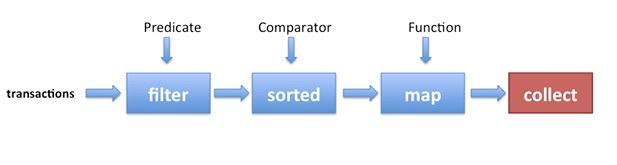
\includegraphics[width=11cm]{pipeline}	
		
	\end{frame}	


	% Stream Processing
	\begin{frame}[fragile]{Lambda Examples: Stream Processing}
		\section{Definition of Lambda}
		
		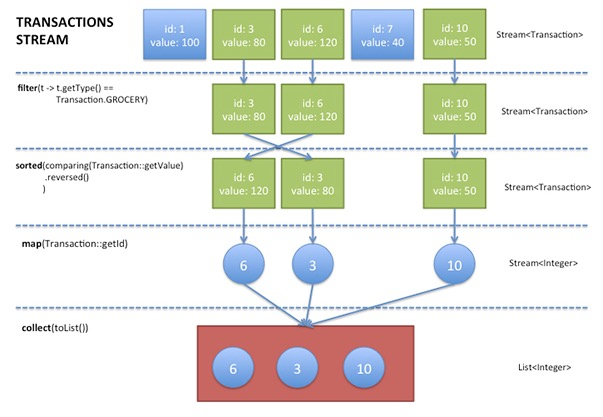
\includegraphics[width=11cm]{processing}	
		
	\end{frame}	
	
	% Stream Processing
	\begin{frame}[fragile]{Lambda Examples: Streams}
		\section{Definition of Lambda}
		
		\begin{itemize}
			\item Stream sources: Arrays, Collections, Generators and I/O Streams, e.g:
				
			\begin{lstlisting}
			try (BufferedReader br = new BufferedReader(new InputStreamReader(is))) {
			    br.lines().forEach(System.out::println);
			}
			catch (Exception e) {
			    System.out.println(e.getMessage());
			}
   			\end{lstlisting}
			
			\item After terminal operation, the stream is considered to be consumed.
			\item The intermediate operations are lazy and always return a new stream. (see Example 6)
				
		\end{itemize}
		
	\end{frame}	
	
	% Examples
	\begin{frame}[fragile]{Lambda Examples: Code Samples}
		\section{Definition of Lambda}

		Some examples (https://github.com/bagdemir/java8-training) : 
		\begin{itemize}
			\item Generators
			\item Comparators
			\item File I/O
			\item Regular Expressions
			\item Reducer
			\item Collectors
			\item Parallel Streams
		\end{itemize}		
	\end{frame}	
	
	% Book Suggestions
	\begin{frame}[fragile]{Lambda Examples: Finish}
		\section{Definition of Lambda}

	\begin{columns}
    	\begin{column}{0.5\textwidth}
			\vspace{0pt}
			\centering
			
\includegraphics[width=3cm]{scalabook} \\
			Functional Programming (in Scala)\\
			
    	\end{column}
    	\begin{column}{0.5\textwidth}
			\vspace{0pt}
			
\includegraphics[width=3cm]{lambdabook}	\\
			Structure and Interpretation of Computer Programs
	  		\end{column}
	\end{columns}
	\end{frame}	
			
	% Links
	\begin{frame}[fragile]{Links}
		\section{Definition of Lambda}
		
		\textbf{Lambda Quick Start}\\
		Oracle.com : http://bit.ly/1eR0we0 \\
		-\\
		\textbf{Streams}\\
		Oracle.com : http://bit.ly/1eh4aZo\\
		Oracle.com : http://bit.ly/1ustKrM\\
		-\\
		\textbf{Contact}\\
		https://github.com/bagdemir\\
		https://twitter.com/ebagdemir\\
		http://www.bagdemir.com\\

	\end{frame}	
	
\end{document}